\documentclass{article}
\usepackage[utf8]{inputenc}
\usepackage{graphicx}
\usepackage{fullpage}
\usepackage[newfloat]{minted}
\usepackage{caption}

\newenvironment{code}{\captionsetup{type=listing}}{}
\SetupFloatingEnvironment{listing}{name=Source Code}

\author{Daniel R. Malone Buoy}
\title{The Lorenz Attractor}
\date{10/31/2017}

\begin{document}
\maketitle
First developed by Edward Lorenz in the early 1960's, the Lorenz Attractor is a set of chaotic solutions to a system of ordinary differential equations.  The system is defined by the following equations\cite{sparrow1982lorenz_equations}:

\begin{equation}
\frac{dx}{dt} = a*(y-x) 
\end{equation}

\begin{equation}
\frac{dy}{dt} = x*(b-z)-y
\end{equation}

\begin{equation}
\frac{dz}{dt} = x*y - c*z
\end{equation}

The Lorenz equations were first developed to represent a rough model of convection in the Earth's atmosphere\cite{tucker1999lorenz}.  In general, "the Lorenz attractor... [describes] the flow of fluid of uniform depth, with an imposed temperature difference, under gravity, with buoyancy, thermal diffusivity, and kinematic viscosity."\cite{tabor1989chaos}.  The chaotic system is incredibly sensitive to the initial conditions.  In systems where the initial conditions differ by small amounts, the results are significantly different.  This observation has been coined as \emph{'The Butterfly Effect'}\cite{dizikes2011butterfly_effect}; which is quite suiting given the graphical representation of the system.

\begin{figure}[h!]
\centering
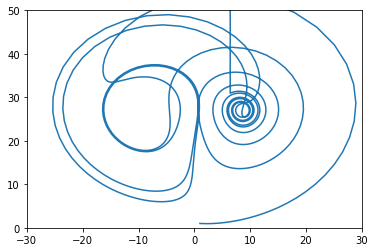
\includegraphics[width=.75\textwidth]{lorenz_Attractor}
\caption{Lorenz Attractor of the form $(0,y,z)$ with initial condition: $f(0,0,0)=[1,1,1]$}
\label{fig:lorenz}
\end{figure}

Given an initial point $(x_0,y_0,z_0)$, the set of solutions form a butterfly shape when plotted.  For the initial point $(1,1,1)$ and with the commonly used coefficients\cite{tabor1989chaos}: $ a=10, b=28,$ and $c=\frac{8}{3}$, the Lorentz system produces a 3-dimensional Lorenz Attractor.  

\begin{figure}[h!]
\centering
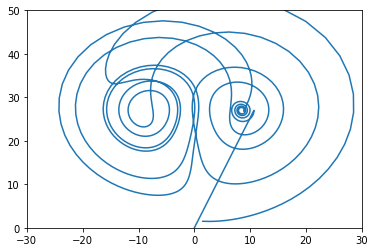
\includegraphics[width=.75\textwidth]{lorenz_Attractor2}
\caption{Lorenz Attractor of the form $(0,y,z)$ with initial condition: $f(0,0,0)=[1.5,1.5,1.5]$}
\label{fig:lorenz2}
\end{figure}

However, fig.\ref{fig:lorenz} represents the 2-dimensional relationship between the parameters $y$ and $z$.  $y$ is plotted along the horizontal axis; whereas, $z$ is plotted along the vertical axis.  Essentially, we have set $x=0$ and have produced a 2-dimensional projection on the $x-plane$.  For the initial point $(1.5,1.5,1.5)$ and with the same coefficients, the Lorentz system produces a quite different projection of a Lorenz Attractor, as shown in fig.\ref{fig:lorenz2}.

The Python code used to produce fig.\ref{fig:lorenz} and fig.\ref{fig:lorenz2} is shown below as Source Code \ref{code:python-code}.  The function \emph{lorenz} takes the parameters: the initial point, $(x_0,y_0,z_0)$ (as a tuple), the constants $a, b, c$, and the change in time $dt$.  The time differential is set at $dt=.01$.  The differentials for $x, y,$ and $z$ are then calculated, and the function returns an array containing the incremental change in each spatial parameter: $x+dx, y+dy$, and $z+dz$.   

In order to generate a visual representation of the system, we must first populate an array with an entry corresponding to each sequential incremental change in the spatial parameters.  For graphical precision, the function is iterated $1000$ times.

From the array, the $y-values$ and $z-values$ can be isolated.  The isolated arrays are then plotted to produce the 2-dimensional projection of the Lorenz Attractors in fig.\ref{fig:lorenz} and fig.\ref{fig:lorenz2}.  For aesthetics, the grid boundaries are set to $-30\leq y\leq 30$ and $0\leq z\leq 50$.

\newpage
\begin{code}
\captionof{listing}{Python Code}
\label{code:python-code}
\begin{minted}{python}
import numpy as np
import matplotlib.pyplot as plt
        
def lorenz(point,dt=.01, a=10, b=28, c=(8/3)):
    
    x=point[0]
    y=point[1]
    z=point[2]

    dx = (a*(y-x))
    dy = (x*(b-z)-y)
    dz = (x*y-z*c)
    
    new_x = x+(dx*dt)
    new_y = y+(dy*dt)
    new_z = z+(dz*dt)
    
    change = np.array([new_x,new_y,new_z])
    
    return change

point = [1,1,1]
steps = 1000
set_of_points = np.empty(((steps+1),3),order='C')
set_of_points[0] = point

for i in range(steps):
    set_of_points[i+1]=lorenz(set_of_points[i])
    
y_values = np.empty(((steps+1),),order='C')
z_values = np.empty(((steps+1),),order='C')

for i in range(steps):
    y_values[i] = set_of_points[i][1]
    z_values[i] = set_of_points[i][2]

plt.plot(y_values, z_values)
plt.axis([-30,30,0,50])
\end{minted}
\end{code}

\newpage
\bibliographystyle{ieeetr}
\bibliography{bibliography_Assignment_6.bib}

\end{document}
